In this chapter, we will describe the hardware and software architecture of the system.
Most of the software is completely decoupled from the hardware part and can be run
on different machines, allowing portability and reusability. On the contrary, the
code is developed only for the specific hardware; mostly the code which is more related
to the specific functionalities of the hardware itself. We will have an overview of the hardware
used and then we will show a general software architecture and its deployment on the
machines involved.

%% Sections of the chapter
\section{Hardware}

The hardware used to run the system is heterogeneous and we will show in details
the machines involved in the project.

First of all, we used a desktop pc as a ground station. It specifics are listed below:
\begin{itemize}
  \item Processor: Intel Core(TM) i5-6500 CPU @ 3.20GHz
  \item Memory: 16 GB
  \item Network: Intel Gigabit CT Network Adapter
  \item Storage: 230 GB
\end{itemize}

On this machine, we run a virtual machine which has the following specifics:
\begin{itemize}
  \item Processor: 1 Core
  \item Memory: 4 GB
  \item Storage 25 GB
  \item Network: Virtual adapter
\end{itemize}

The flying machines involved in the mission are of two kinds, but both adopt the
same general configuration, even with different hardware. Indeed, they are equipped
with a flight control unit connected with a companion microcomputer by the serial port
The microcomputer communicates with the ground station using the Wifi.

\subsection{Pixfalcon}
The flight control unit adopted it the Pixfalcon (figure \ref{fig:hardware_pixfalcon})
which belongs to the family of the Pixhawk \cite{pixhawk}.

\begin{figure}[h]
\centering
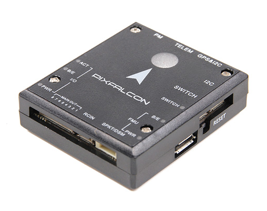
\includegraphics[width=0.35\textwidth]{chapters/chapter-03/figures/hardware_pixfalcon.png}
\caption{Pixfalcon board}
\label{fig:hardware_pixfalcon}
\end{figure}

Its specifications are the following:
\begin{itemize}
  \item Main System-on-Chip: STM32F427
        \begin{itemize}
          \item CPU: 180 MHz ARM Cortex M4 with single-precision FPU
          \item RAM: 256 KB SRAM (L1)
        \end{itemize}

  \item Failsafe System-on-Chip: STM32F100
        \begin{itemize}
          \item CPU: 24 MHz ARM Cortex M3
          \item RAM: 8 KB SRAM
        \end{itemize}

  \item Wifi: ESP8266 external
  \item GPS: U-Blox 7/8 (Hobbyking) / U-Blox 6 (3D Robotics)
  \item Connectivity:
    \begin{itemize}
      \item 1x I2C
      \item 1x CAN (2x optional)
      \item 1x ADC
      \item 4x UART (2x with flow control)
      \item 1x Console
      \item 8x PWM with manual override
      \item 6x PWM / GPIO / PWM input
      \item S.BUS / PPM / Spektrum input
      \item S.BUS output
    \end{itemize}
\end{itemize}

\subsection{Intel Edison}
The companion computers are of two types.
The first kind is the Intel Edison \cite{edison} (figure \ref{fig:hardware_edison})
which is a general purpose computer.

\begin{figure}[h]
\centering
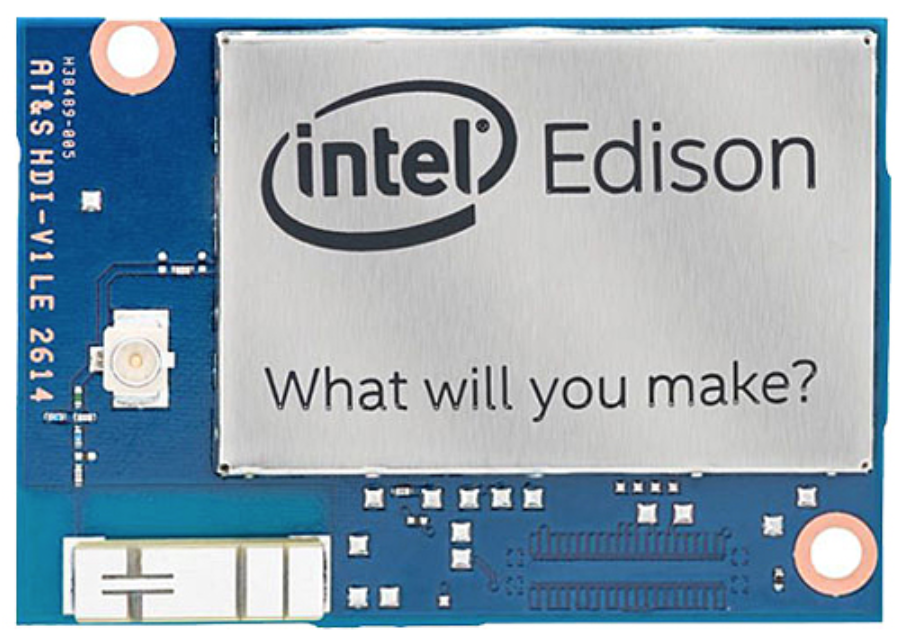
\includegraphics[width=0.35\textwidth]{chapters/chapter-03/figures/hardware_edison.png}
\caption{Edison board}
\label{fig:hardware_edison}
\end{figure}

The specifications are the following:

\begin{itemize}
  \item Atom 2-Core (Silvermont) x86 @ 500 MHz
  \item Memory: LPDDR3 1 GB
  \item Storage: 4 GB EMMC
\end{itemize}

\subsection{RaspberryPi Zero}
The second kind of companion is the RaspberryPi Zero \cite{raspberry}
(figure \ref{fig:hardware_raspberry}).

\begin{figure}[h]
\centering
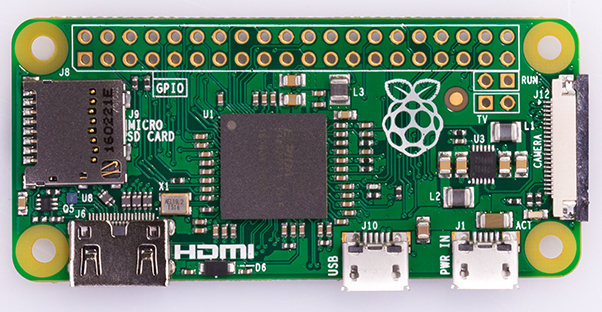
\includegraphics[width=0.35\textwidth]{chapters/chapter-03/figures/hardware_raspberry.jpg}
\caption{RaspberryPi Zero board}
\label{fig:hardware_raspberry}
\end{figure}

The specifications are the following:

\begin{itemize}
  \item Processor:
        \begin{itemize}
          \item Broadcom BCM2835
          \item contains an ARM1176JZFS (ARM11 using an ARMv6-architecture core)
        \end{itemize}

  \item Memory: 512MB LPDDR2 SDRAM

  \item USB On-The-Go port
  \item Mini HDMI
  \item 40pin GPIO header
  \item CSI camera connector (newer version from May 2016)
\end{itemize}

\subsection{Motive Optitrack}
The motion capture system is Motive Optitrack \cite{optitrack}.
We use eight Optitrack Prime 13 cameras \cite{prime13},
arranged on a square as show in the figure \ref{fig:camera_square}.

\begin{figure}[h]
\centering
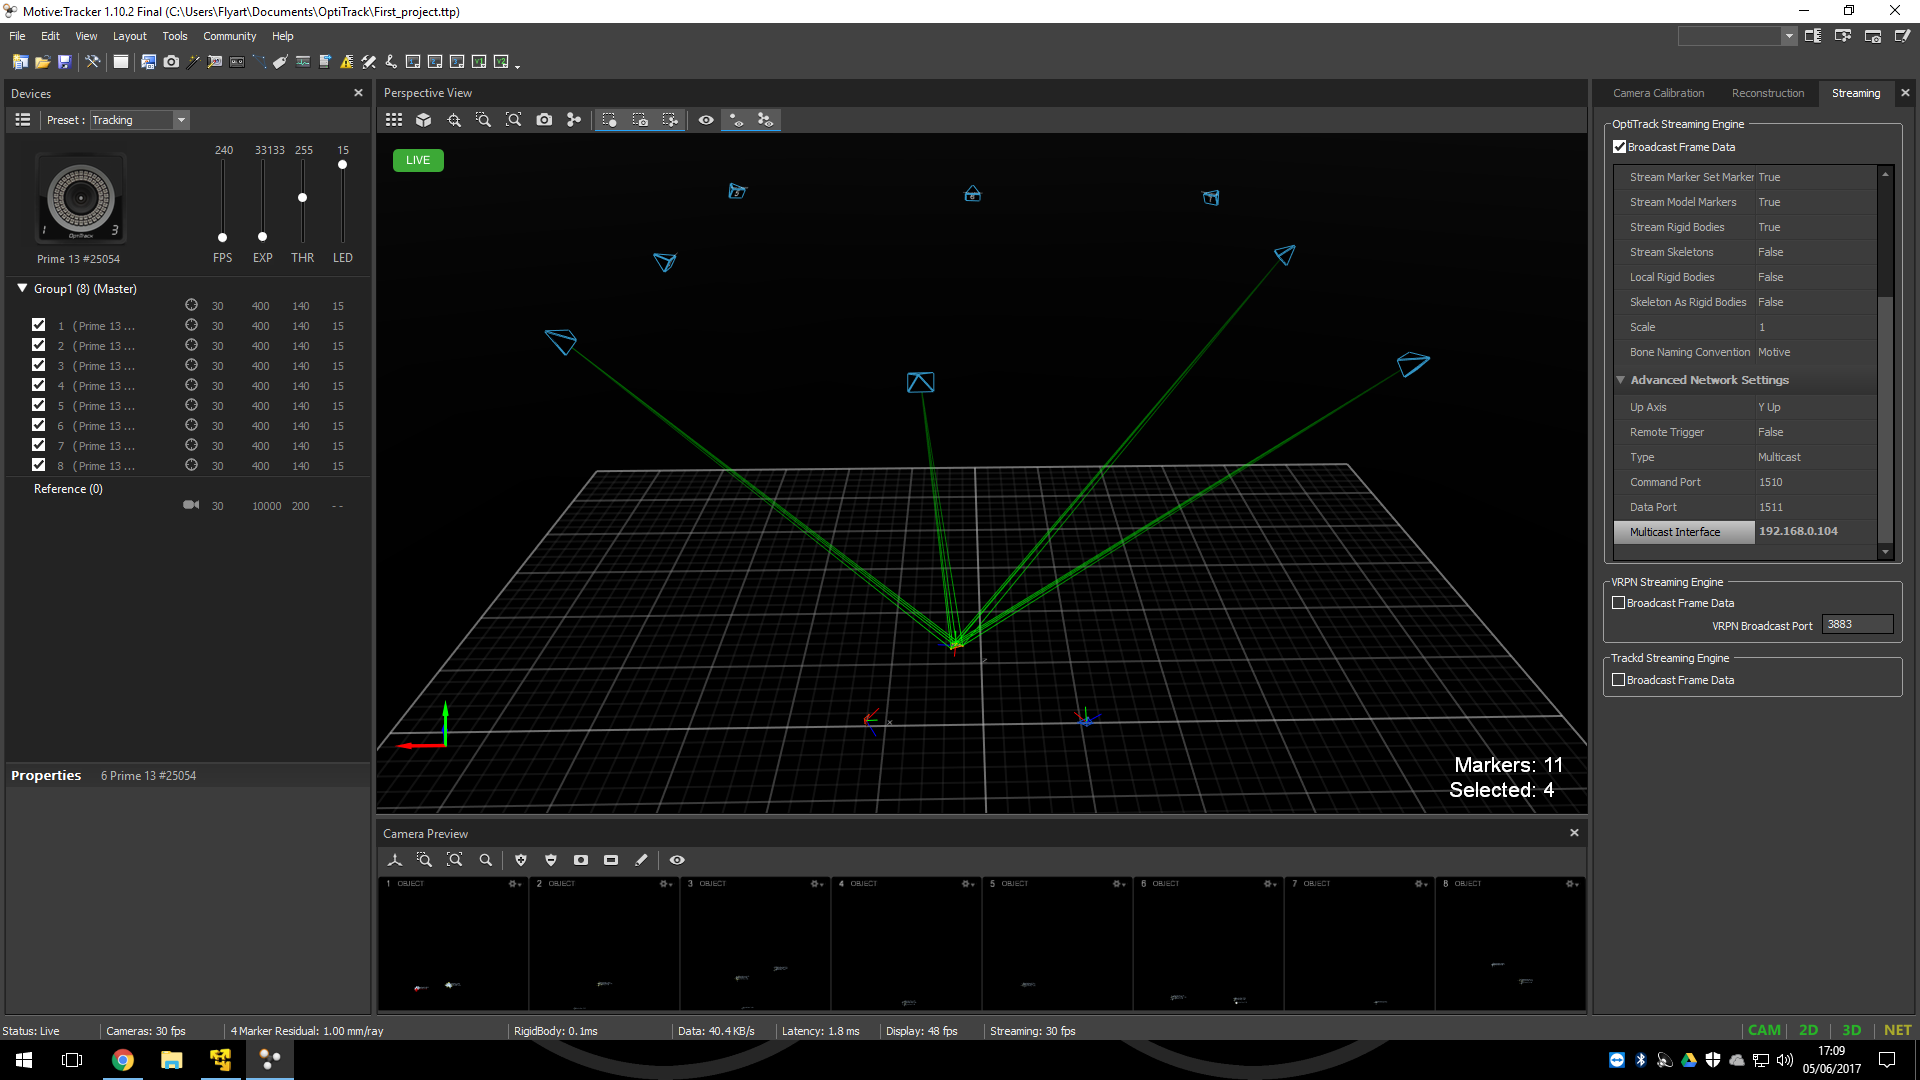
\includegraphics[width=1.0\textwidth]{chapters/chapter-03/figures/cameras_square.png}
\caption{Motive Optitrack screenshot}
\label{fig:camera_square}
\end{figure}

The cameras are connected to a Netgear Prosafe 28PT GE POE \cite{netgear} switch using
Gigabit Ethernet cables.

In order to be visible by the Optitrack system, every drone must be equipped with
markers (figure \ref{fig:marker}), with different configurations,
which make possible the diversification of all the drones. %TODO photo markers

\begin{figure}[h]
\centering
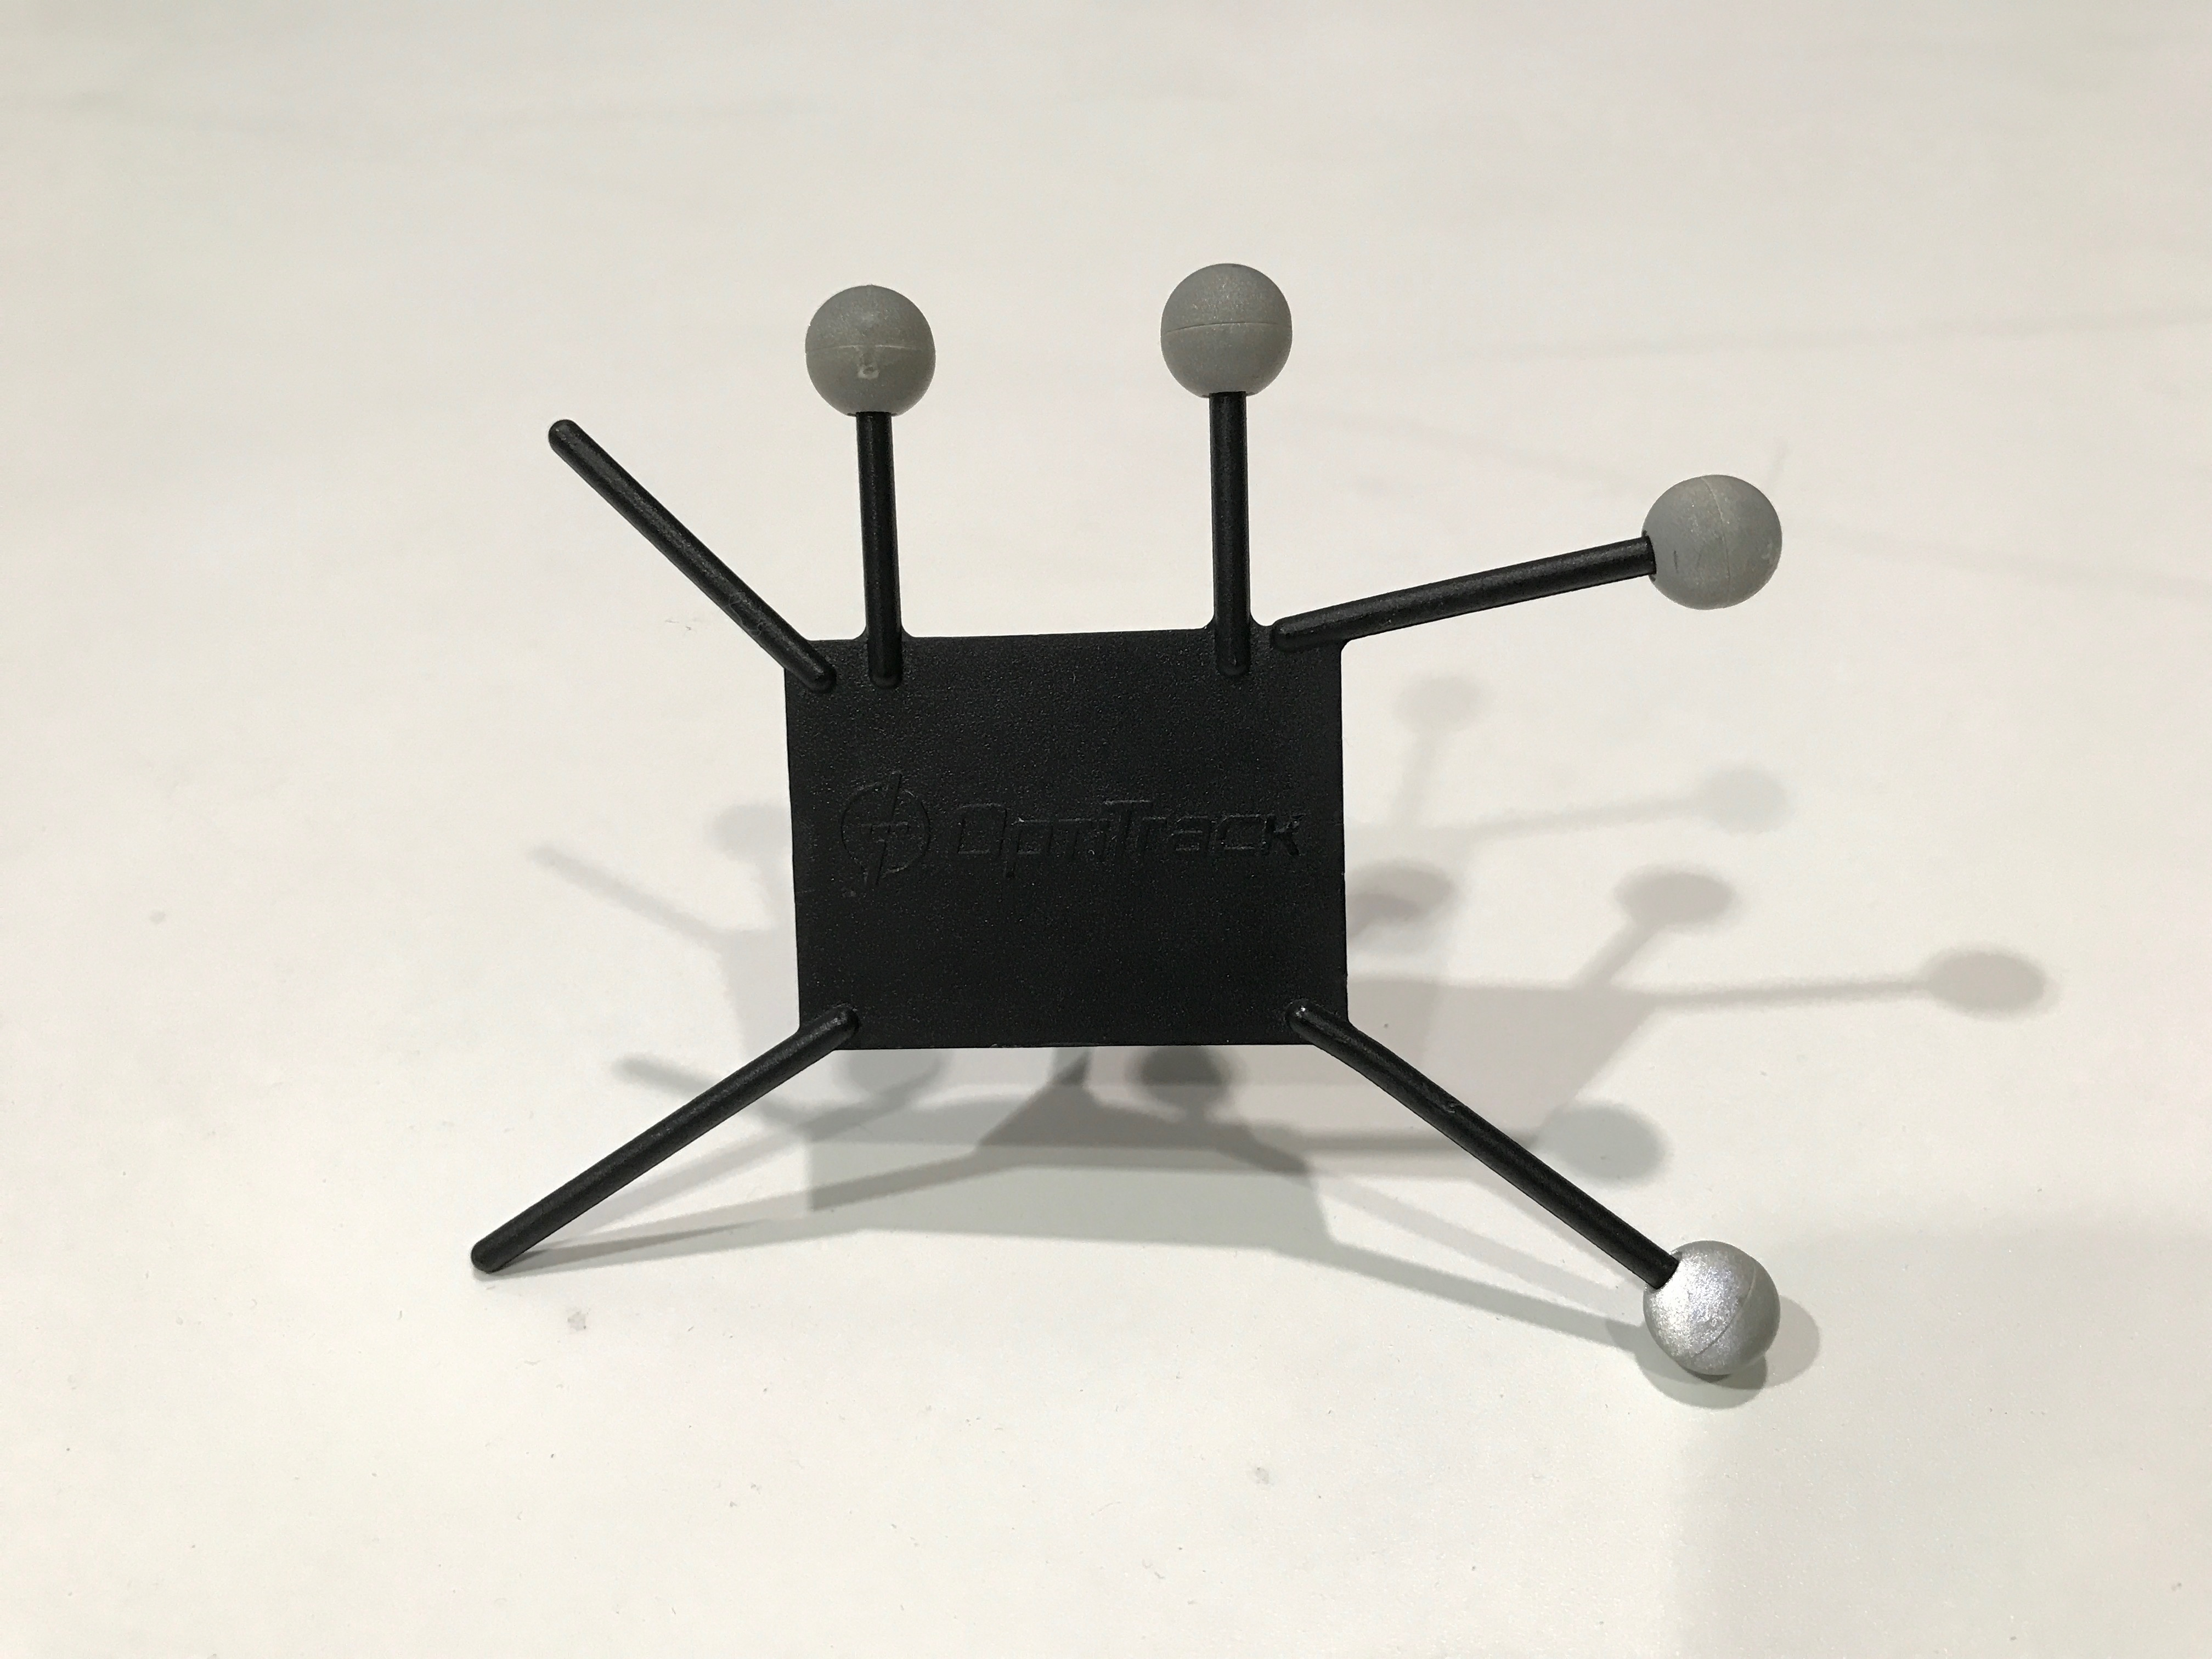
\includegraphics[width=0.7\textwidth]{chapters/chapter-03/figures/marker.jpg}
\caption{Optitrack marker}
\label{fig:marker}
\end{figure}

The two models of drone which we will use are presented in the figures \ref{fig:ant1}
and \ref{fig:hexa}. The first one is the Ant model, which is equipped with the Raspberry
Pi Zero and the Pixfalcon. It is a tiny drones which weights about 200g.
The second one is the Hexa model. It is provided with the Intel Edison board and
the Pixfalcon. It is larger and its diameters is about 40cm long.
As we can see from the figures, the Ant model has four propellers, while the Hexa
is provided with six ones.

\begin{figure}[!htb]
\minipage{0.5\textwidth}
  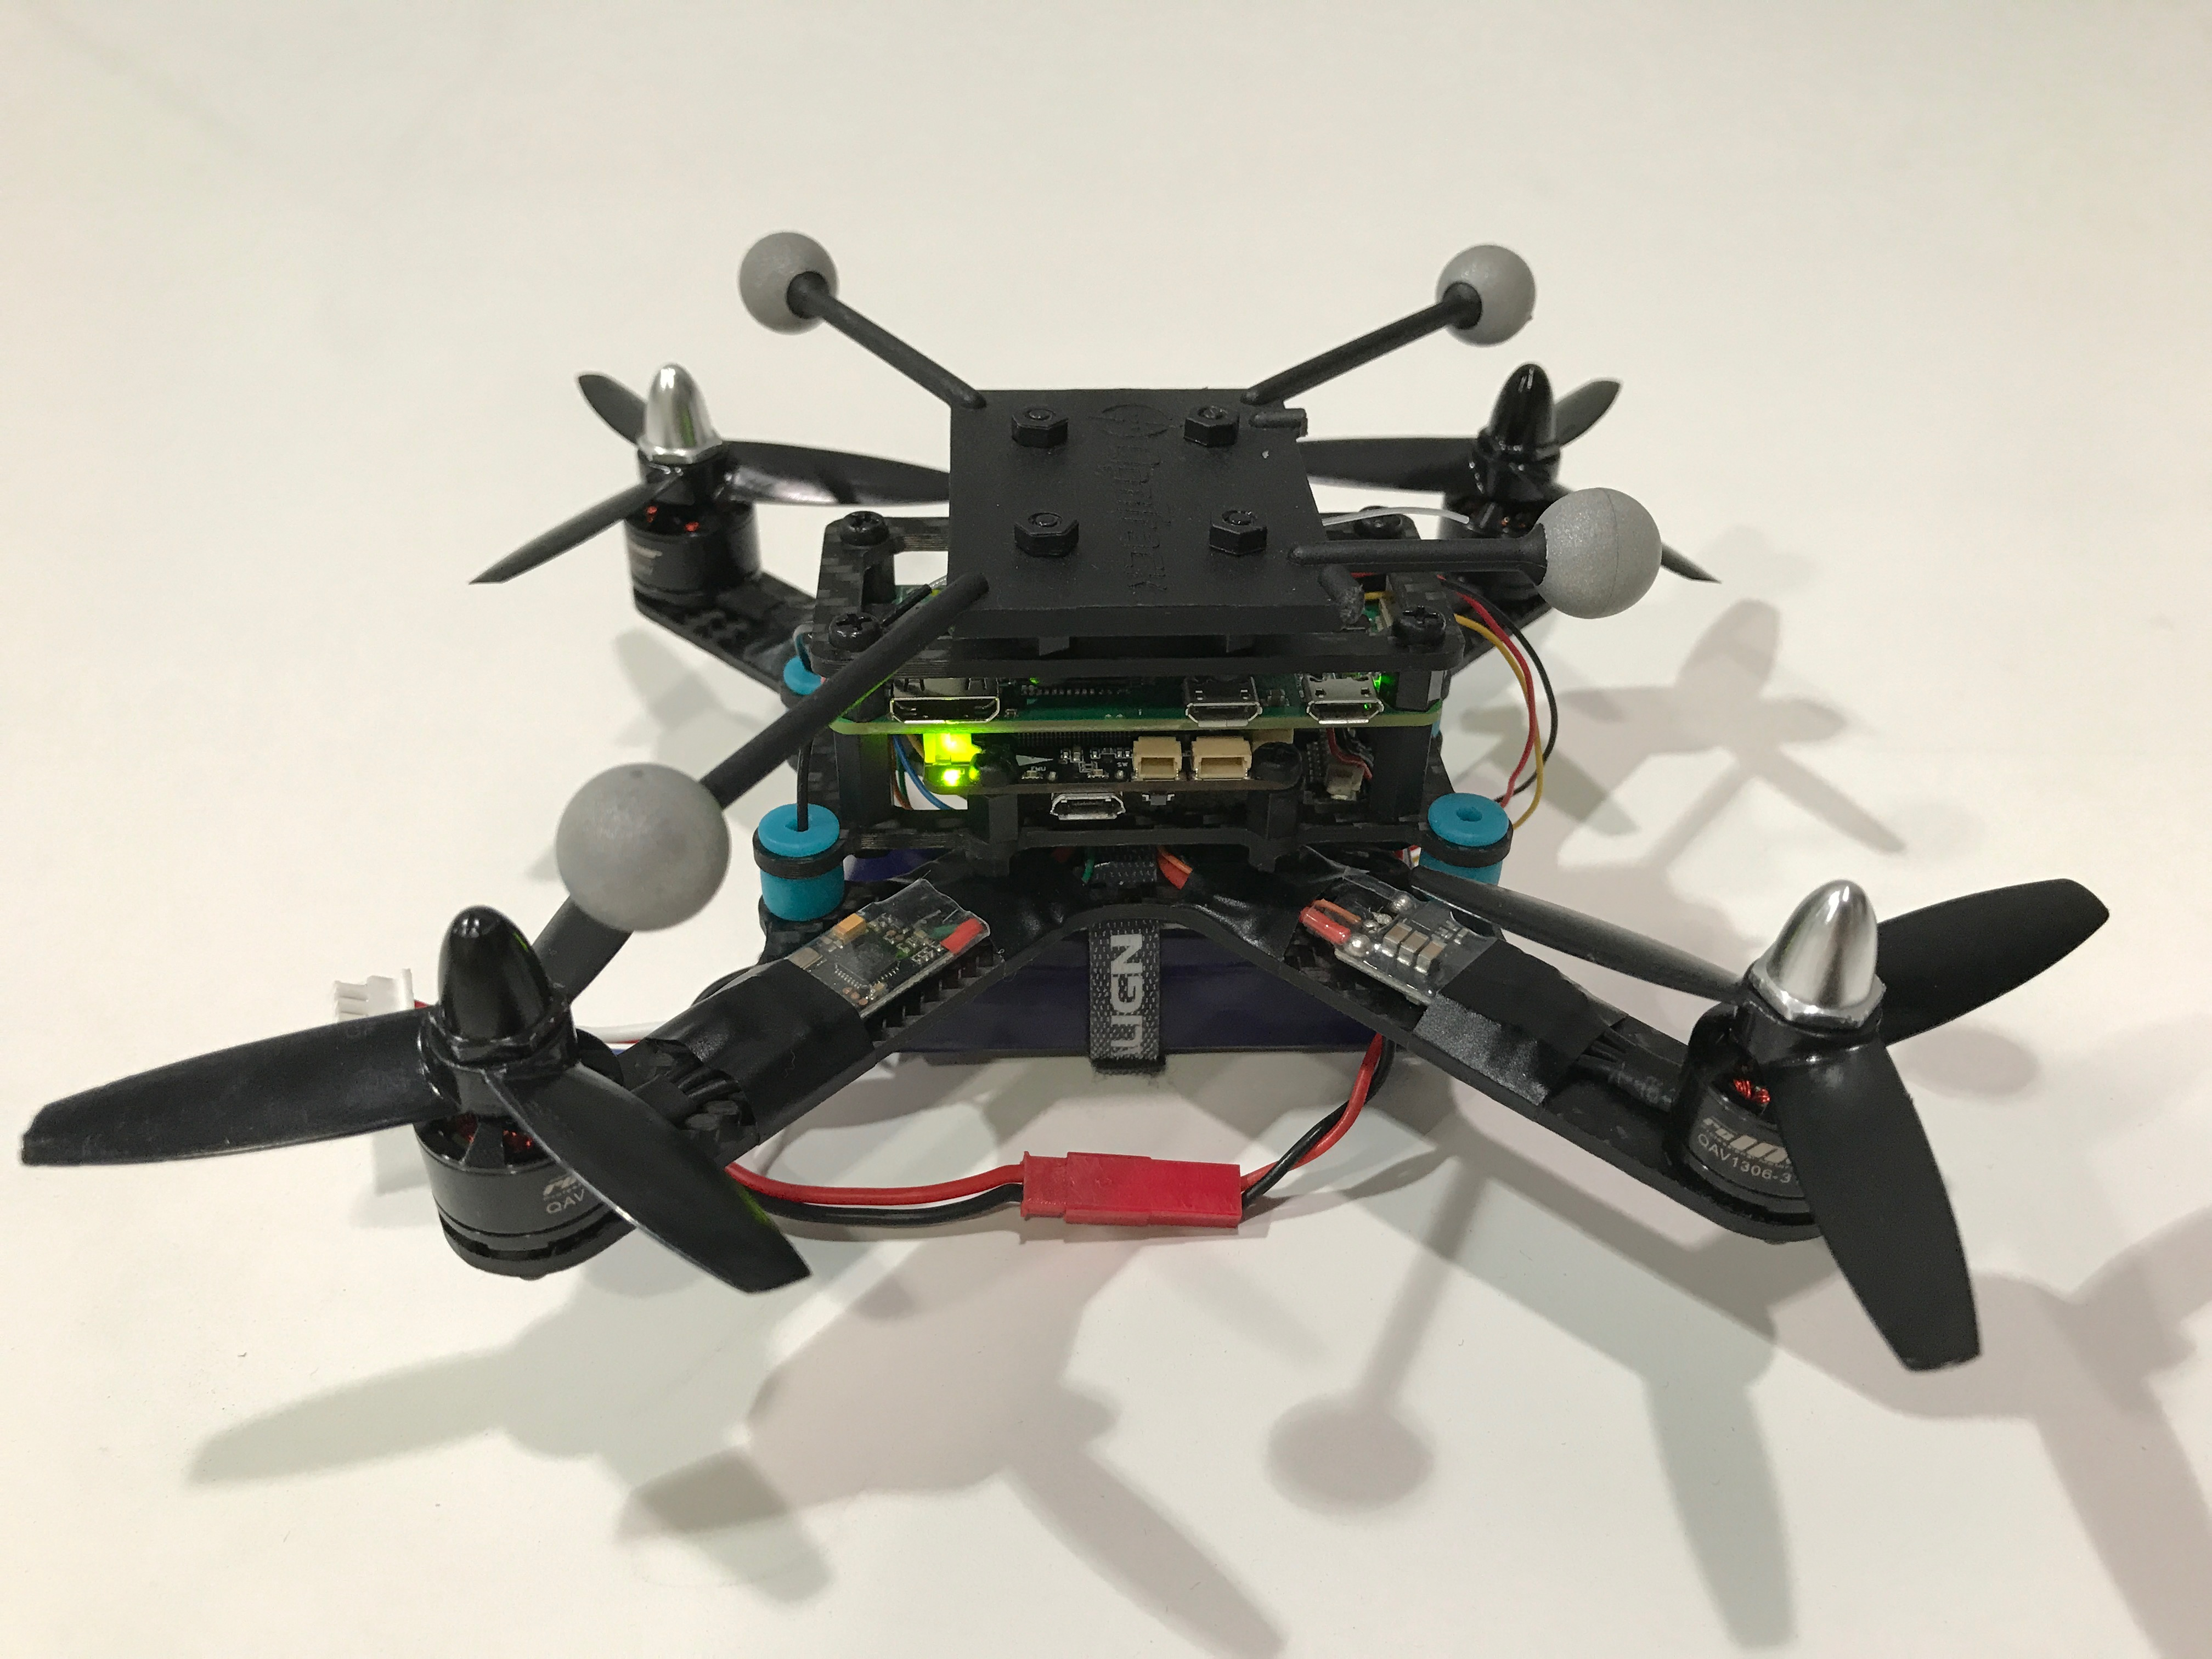
\includegraphics[width=\linewidth]{chapters/chapter-03/figures/ant1_1.jpg}
\endminipage\hfill
\minipage{0.5\textwidth}
  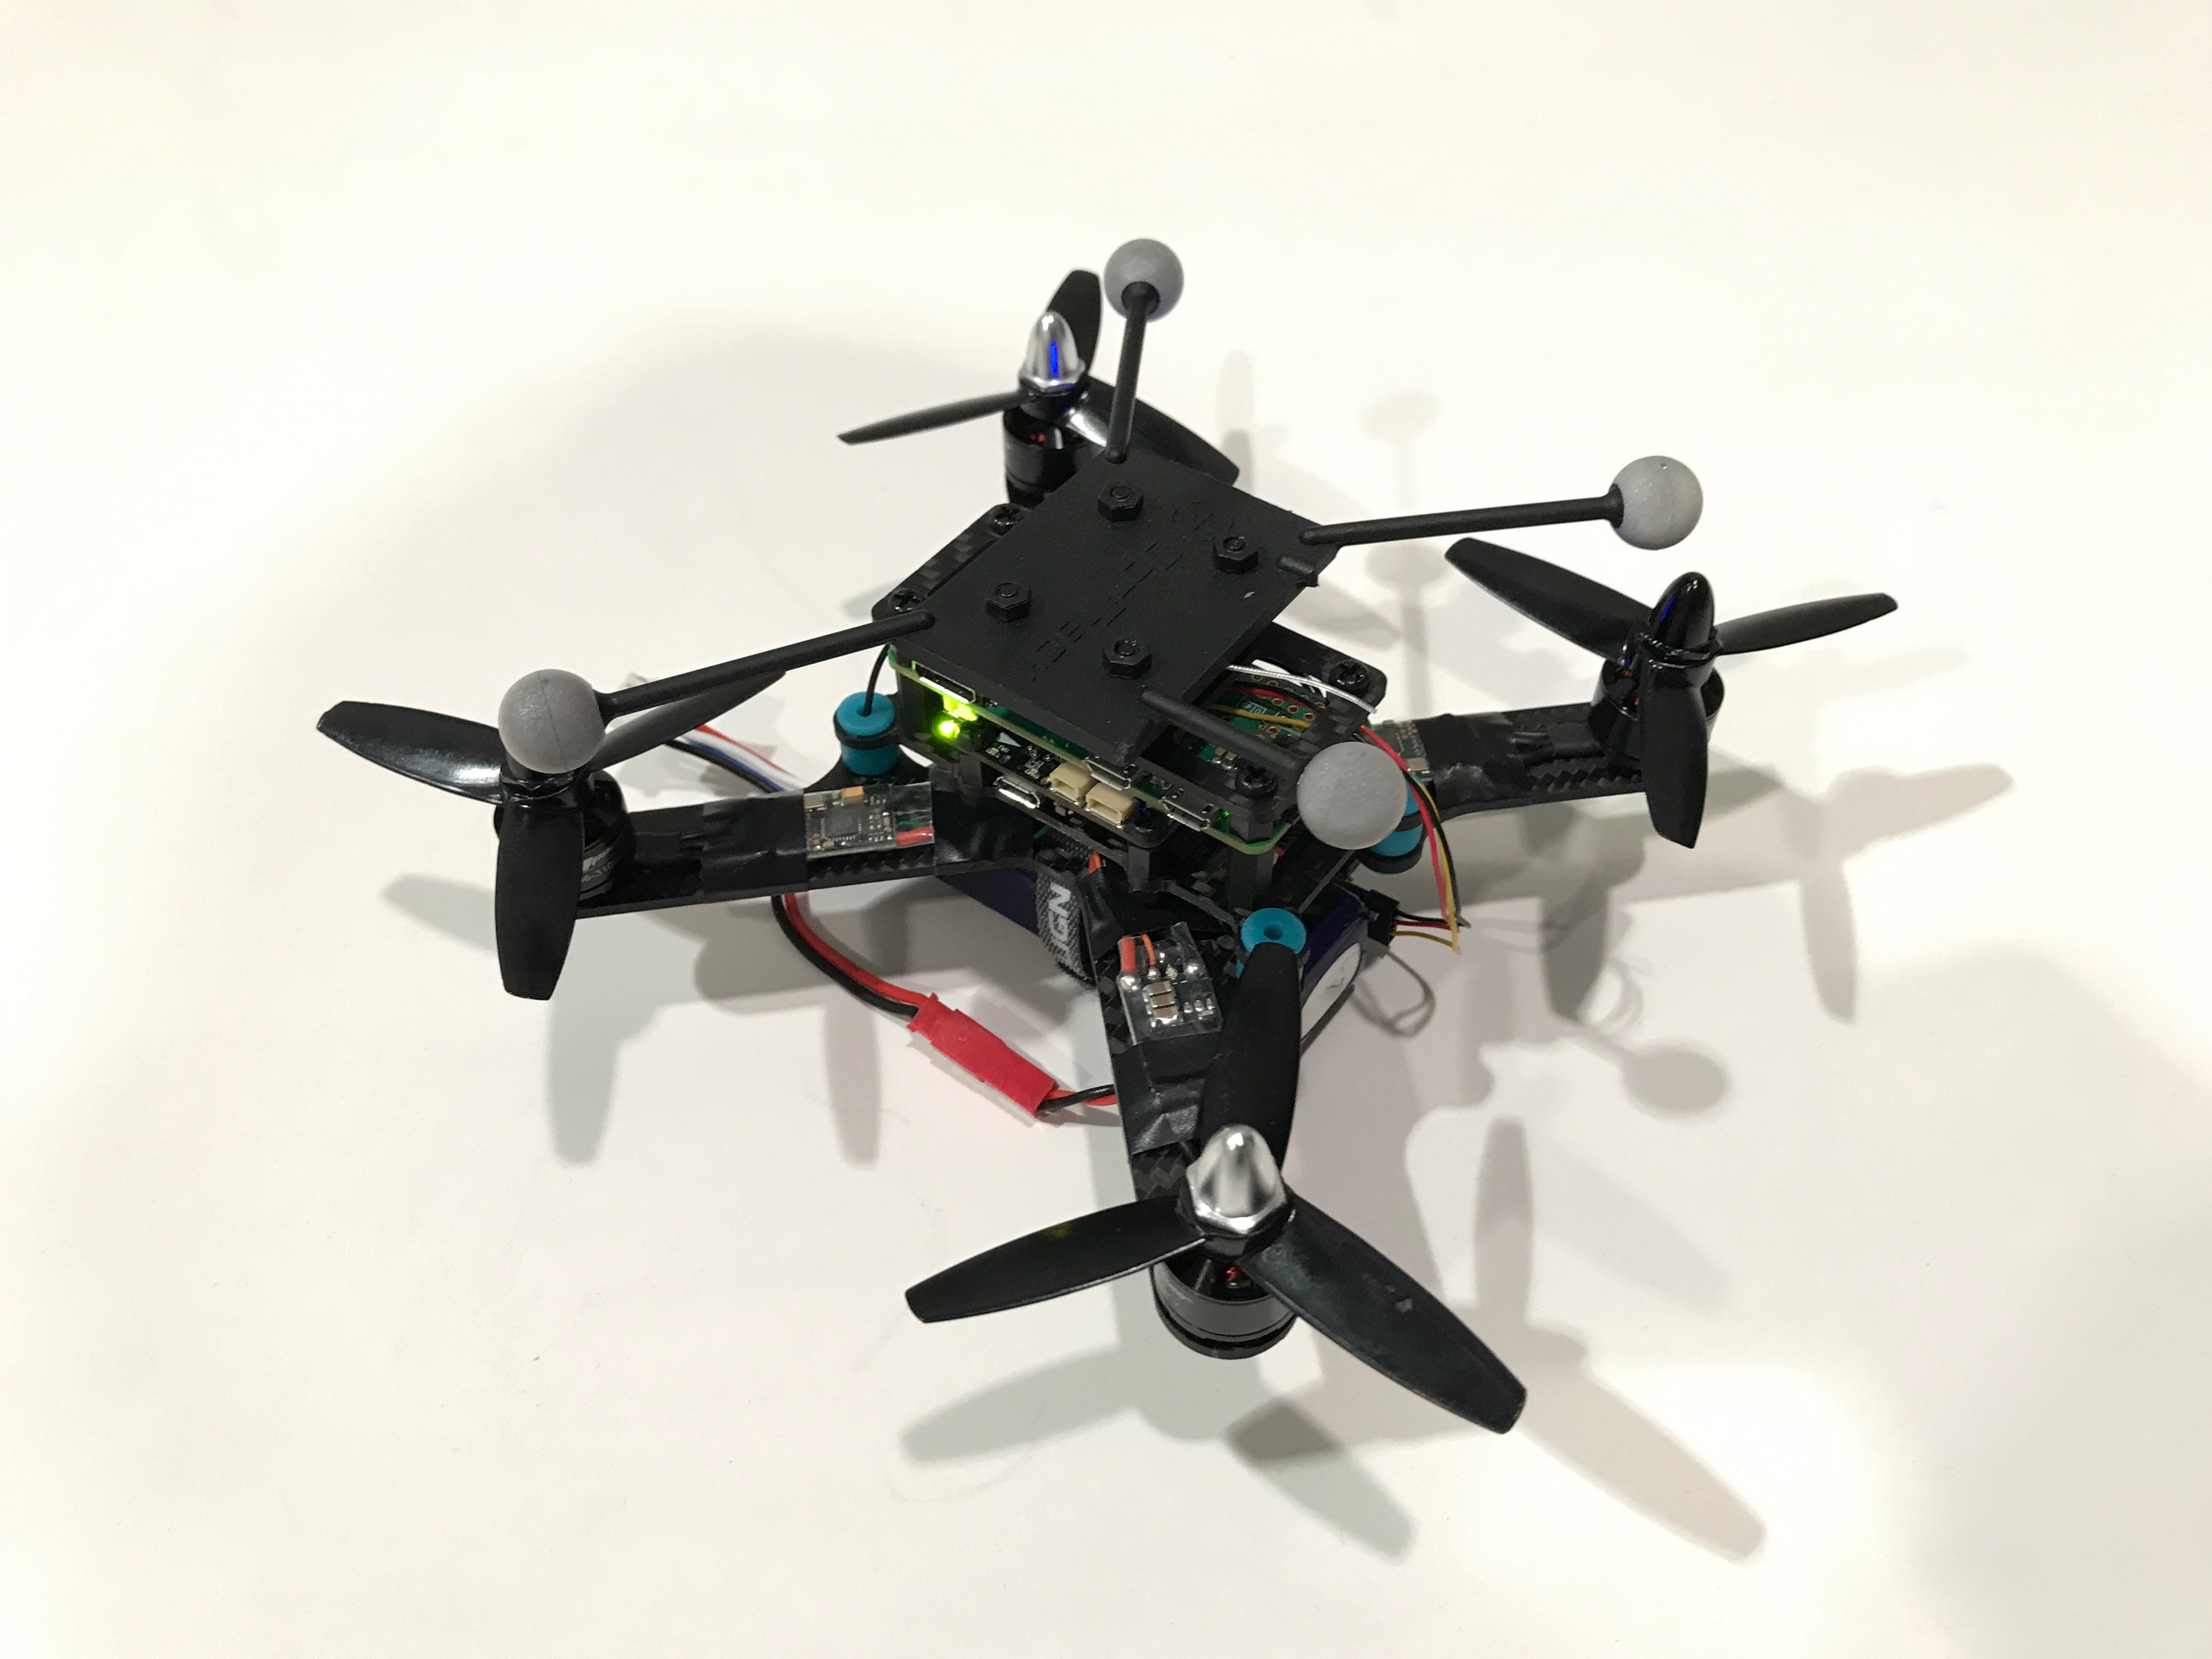
\includegraphics[width=\linewidth]{chapters/chapter-03/figures/ant1_2.jpg}
\endminipage
\caption{Ant drone}
\label{fig:ant1}
\end{figure}

\begin{figure}[!htb]
\minipage{0.5\textwidth}
  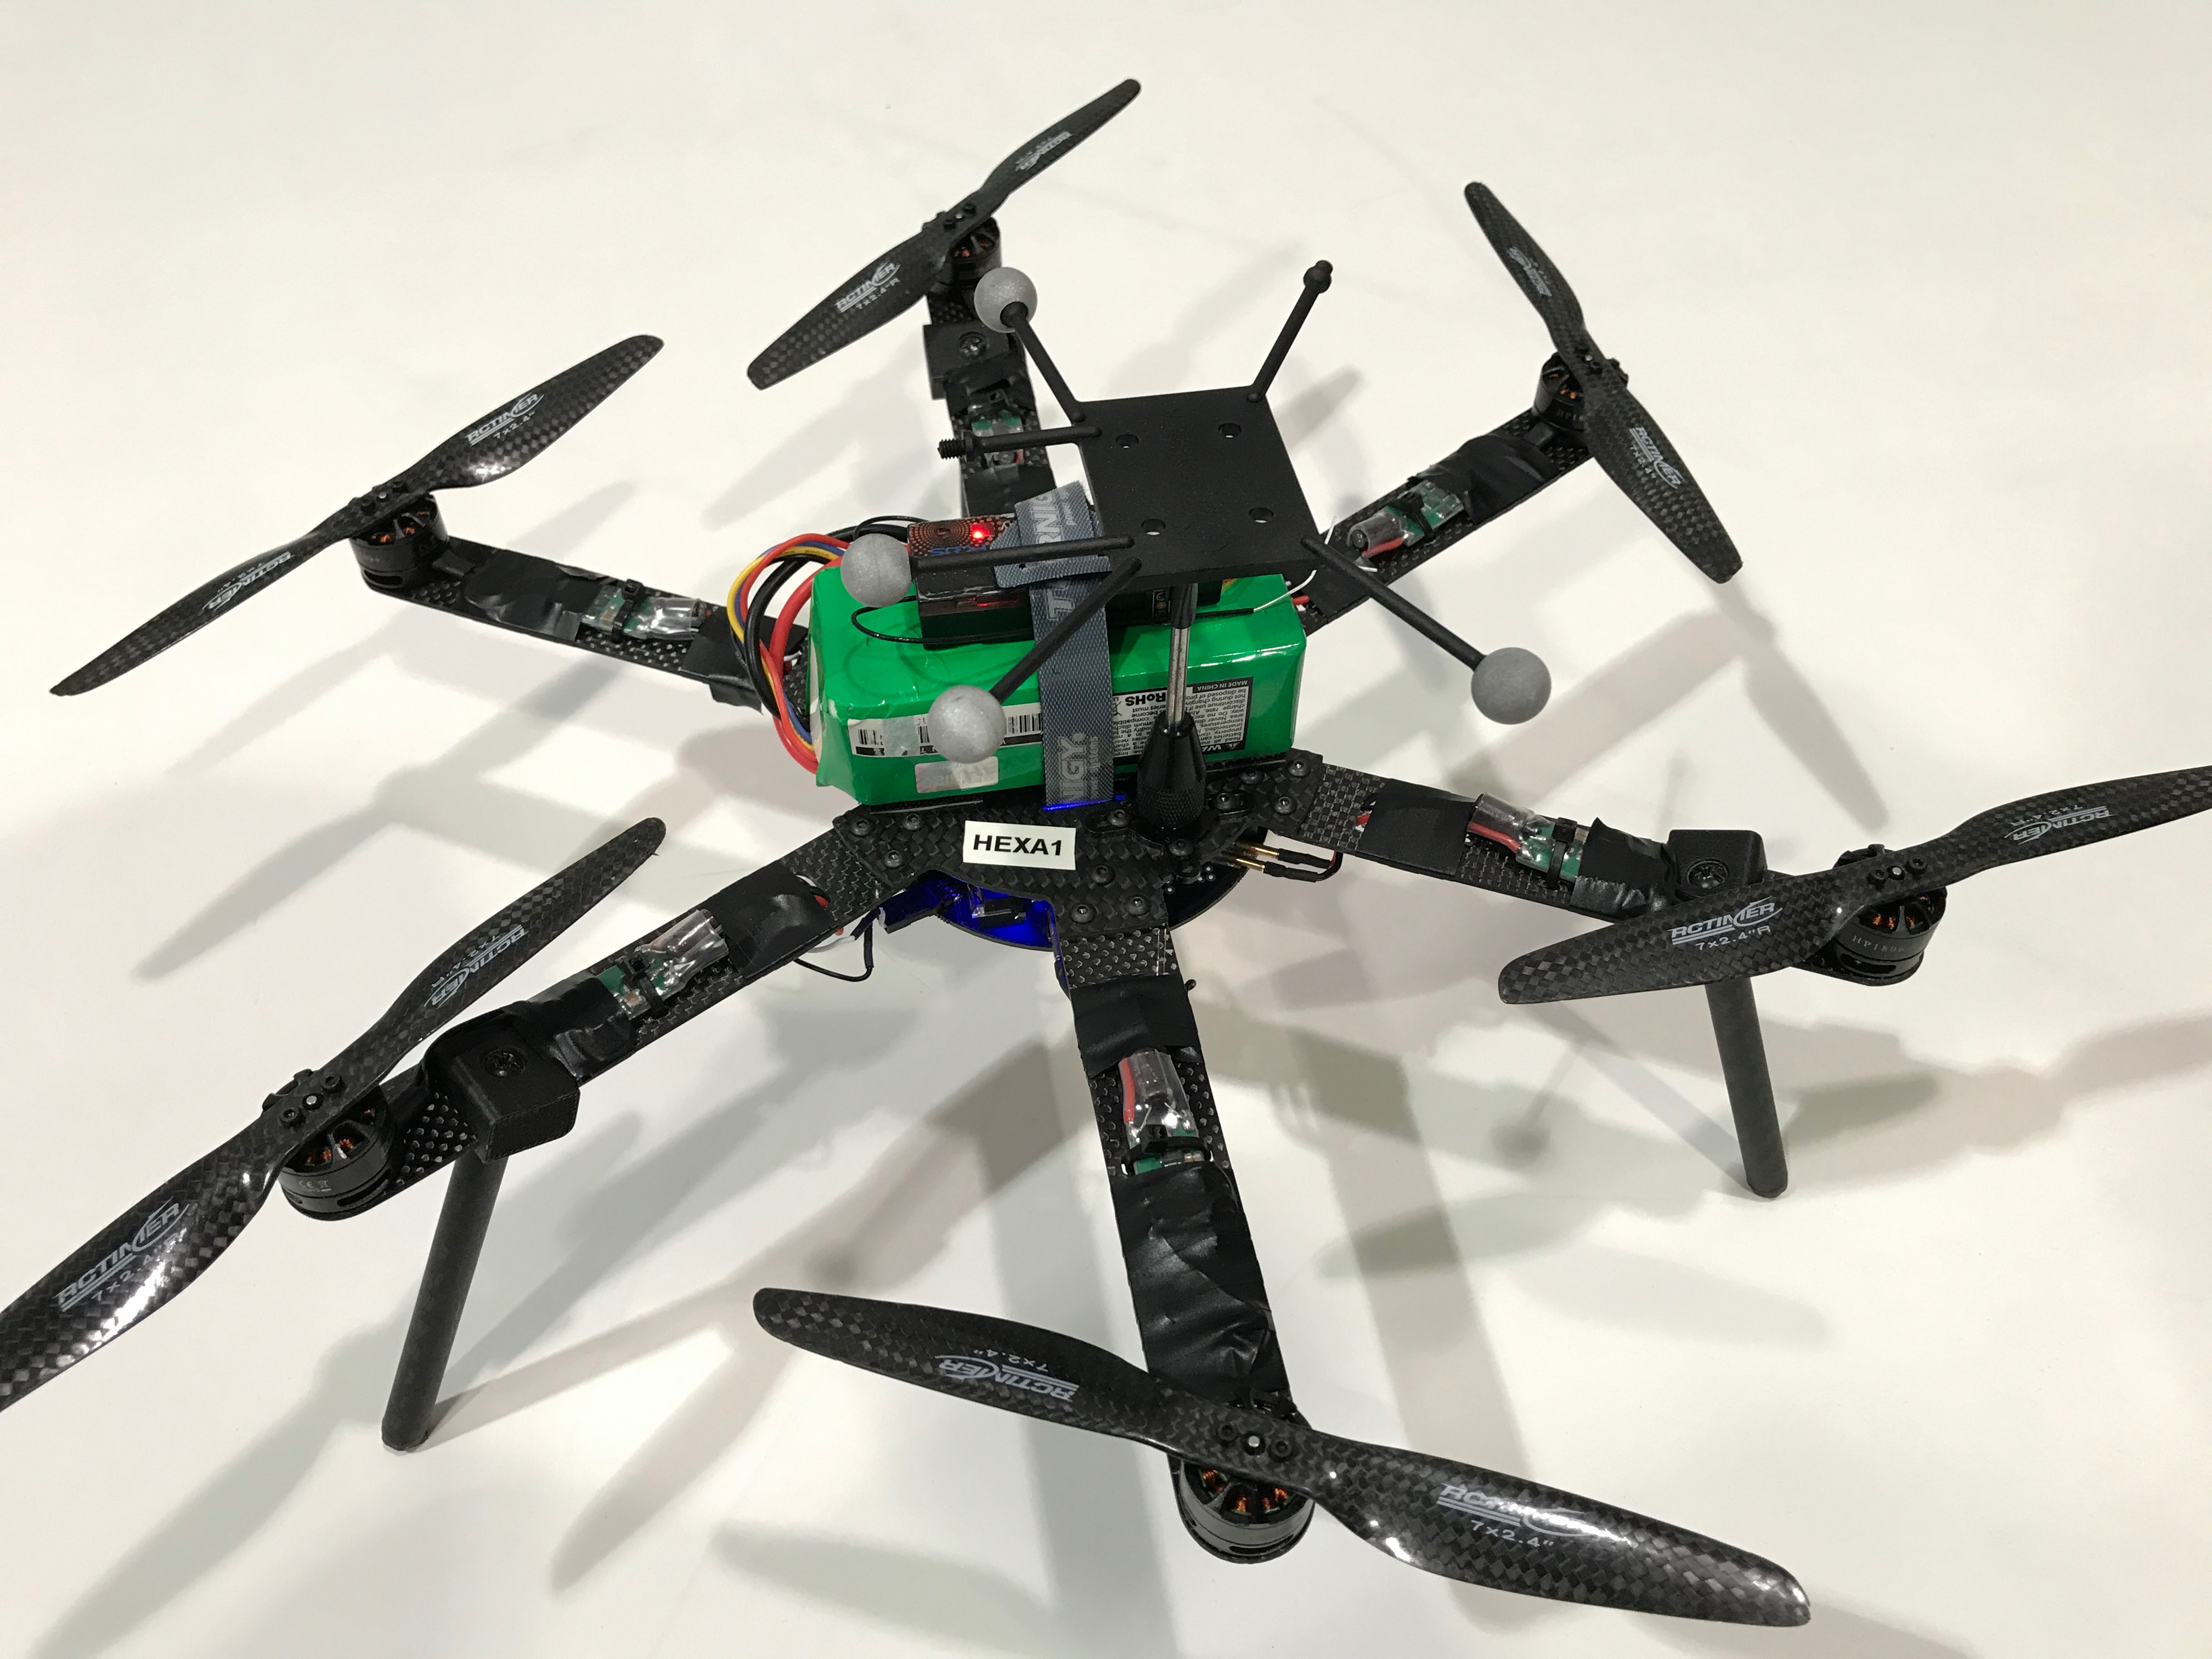
\includegraphics[width=\linewidth]{chapters/chapter-03/figures/hexa_1.jpg}
\endminipage\hfill
\minipage{0.5\textwidth}
  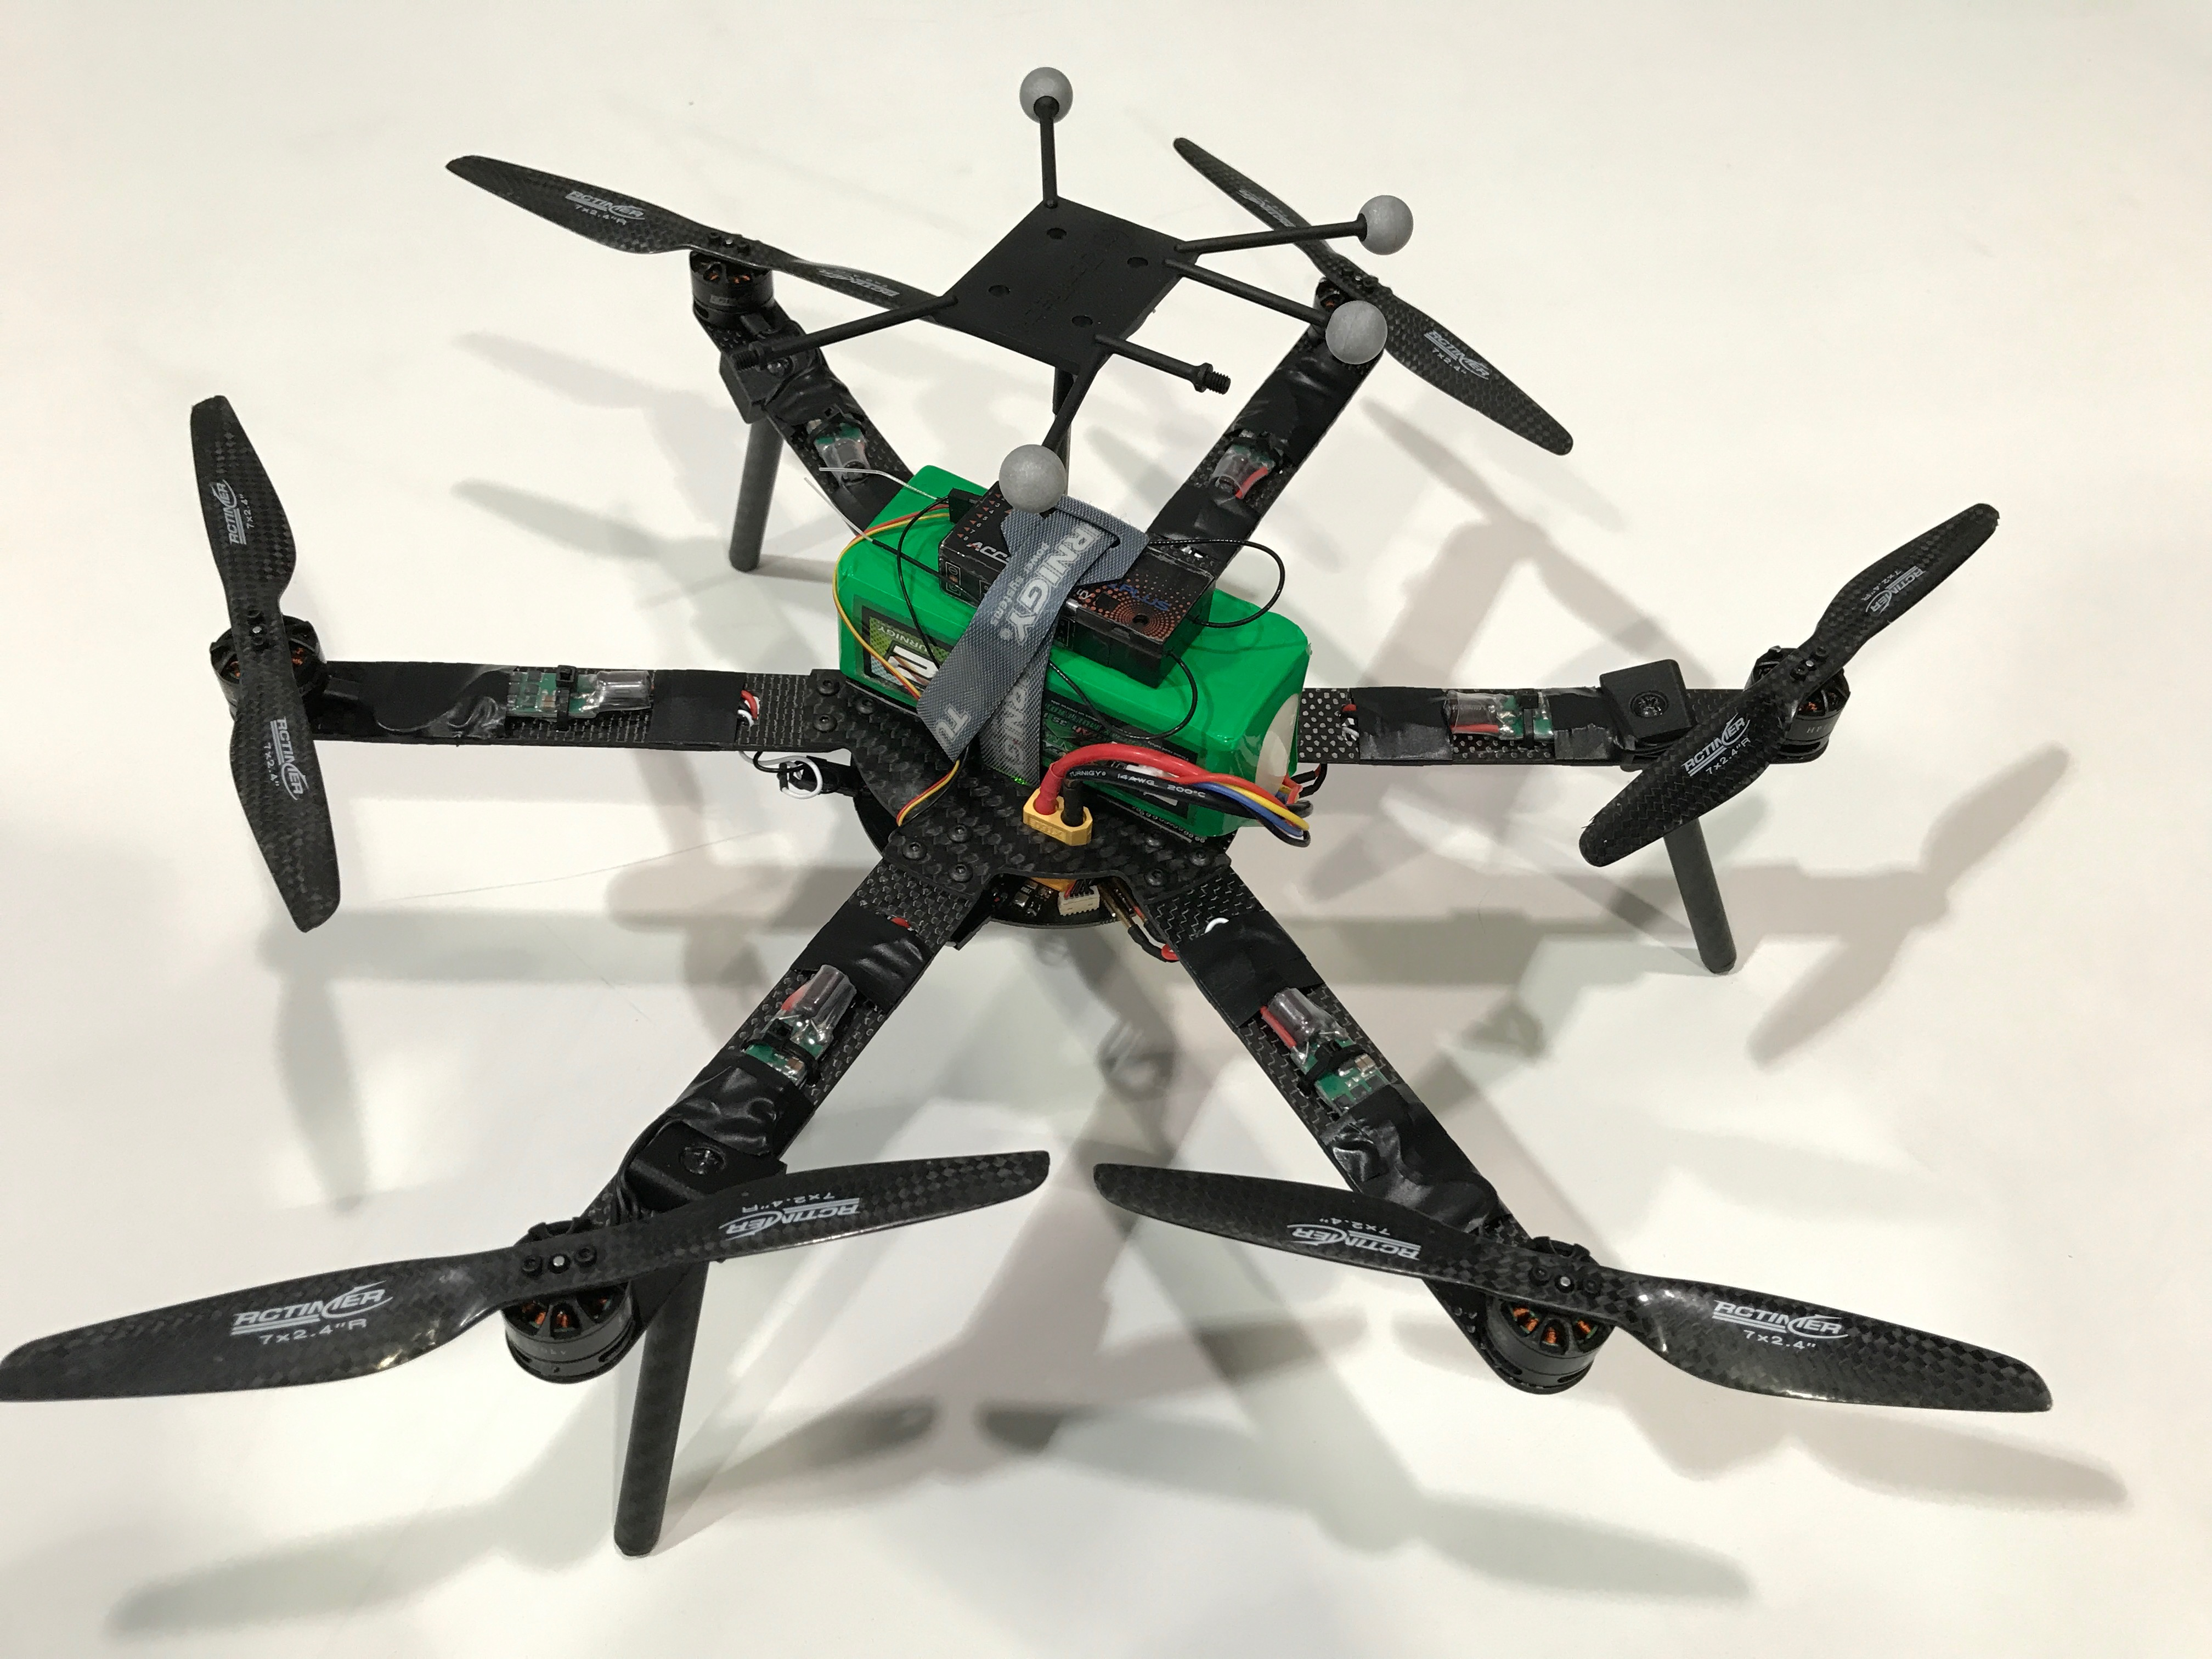
\includegraphics[width=\linewidth]{chapters/chapter-03/figures/hexa_2.jpg}
\endminipage
\caption{Hexa drone}
\label{fig:hexa}
\end{figure}


\section{Software}

We now list all the software adopted in order to execute the algorithm
in a real environment and in the simulated one.

The principal software used to manage the distributed architecture is ROS Kinetic
Kame \cite{ros}.
ROS is a robotic middleware which can manage in a distributed environment more
machines with a structure which is mainly publisher-subscriber.
The central part of the ROS architecture is a node called ROS core, which manages
the topics of the system and the subscriptions.
The ROS core offers also other functionalities such as the Parameter Server or the
possibility to advertise services.
The Parameter Server is a central infrastructure which is responsible for storing
configuration parameters loaded by the nodes of the system.
These parameters can be retrieved by the nodes and used whether needed.
Instead, a ROS service is a sort of remote function call. One node can advertise
the service, which can be called by any other nodes. The call is synchronous and
so the caller is blocked until the callee has executed its callback function.
ROS architecture is based on queues and threads and most of the provided functions
hide part of the implementations of these tools.


\subsection{Ground station}
The ground station runs Windows 10 Pro \cite{windows} and the software used to virtualize a
Desktop machine is VMware \cite{vmware}.
On the virtual machine is installed Ubuntu 16.04 LTS \cite{ubuntu} in order to run software
needed and available only for Unix systems.

On Windows operative system we launch the Motive Optitrack software \cite{optitrack},
which allows to calibrate and control the cameras. It also provides the streaming of
the positions of the markers identified by the cameras and sends it to the Ubuntu
operative system.
Here, the information is converted by a ROS node and sent through the ROS topics,
which are read by the drones. In this way, each drone knows exactly its position.
This node is an open source node called Mocap which can be found on GitHub \cite{mocap}.
On Ubuntu side, we launch the ROS core, which manages all the ROS nodes and topics.

\subsection{Raspberry Pi Zero}
The Raspberry Pi Zero executes a dedicated version of Debian operative system,
which is Raspbian. The version used is Raspbian Jessie 4.4 \cite{raspbian}.

\subsection{Intel Edison}
The Intel Edison runs a version of Debian called Jubilinux version 0.1.1 \cite{jubilinux}.

\subsection{Both companions}
Both companions, the Raspberry and the Edison, are provided with ROS Kinetic and
both have to execute some ROS nodes in order to communicate with the others.

First of all, they run Mavros nodes \cite{mavros}.
This kind of node can be downloaded from GitHub and manages the conversion of the
information taken from the ROS topics to the serial port and vice versa. Indeed,
the ROS messages are converted into Mavlink messages and sent through the serial
to the Pixfalcon autopilot. The same is done for the Mavlink messages from the
autopilot, which are published on ROS topics.

The second kind of ROS node run by the companions, is a custom consensus node, which
loads the desired trajectory and sends the next set point to the Mavros node.
This node will be analyzed in details in the chapter \ref{chap:consensus_node}.

\subsection{Pixfalcon}
The Pixfalcon autopilot is flashed with an open source firmware,
the PX4 Pro Autopilot \cite{px4}, which is downloadable from GitHub.
The release used is the v1.5.5.

\subsection{Additional software}
We use Matlab R2016\_B \cite{matlab} to the data process and to graph plot. We also use it to validate
some theoretical results.

This document is written in  \LaTeX \ \cite{latex} and the code IDE used is Atom \cite{atom},
while the versioning control platform used are GitHub \cite{github} and GitLab \cite{gitlab}.

